% Options for packages loaded elsewhere
\PassOptionsToPackage{unicode}{hyperref}
\PassOptionsToPackage{hyphens}{url}
%
\documentclass[
]{article}
\usepackage{lmodern}
\usepackage{amssymb,amsmath}
\usepackage{ifxetex,ifluatex}
\ifnum 0\ifxetex 1\fi\ifluatex 1\fi=0 % if pdftex
  \usepackage[T1]{fontenc}
  \usepackage[utf8]{inputenc}
  \usepackage{textcomp} % provide euro and other symbols
\else % if luatex or xetex
  \usepackage{unicode-math}
  \defaultfontfeatures{Scale=MatchLowercase}
  \defaultfontfeatures[\rmfamily]{Ligatures=TeX,Scale=1}
\fi
% Use upquote if available, for straight quotes in verbatim environments
\IfFileExists{upquote.sty}{\usepackage{upquote}}{}
\IfFileExists{microtype.sty}{% use microtype if available
  \usepackage[]{microtype}
  \UseMicrotypeSet[protrusion]{basicmath} % disable protrusion for tt fonts
}{}
\makeatletter
\@ifundefined{KOMAClassName}{% if non-KOMA class
  \IfFileExists{parskip.sty}{%
    \usepackage{parskip}
  }{% else
    \setlength{\parindent}{0pt}
    \setlength{\parskip}{6pt plus 2pt minus 1pt}}
}{% if KOMA class
  \KOMAoptions{parskip=half}}
\makeatother
\usepackage{xcolor}
\IfFileExists{xurl.sty}{\usepackage{xurl}}{} % add URL line breaks if available
\IfFileExists{bookmark.sty}{\usepackage{bookmark}}{\usepackage{hyperref}}
\hypersetup{
  pdftitle={Problemas variables aleatorias continuas},
  hidelinks,
  pdfcreator={LaTeX via pandoc}}
\urlstyle{same} % disable monospaced font for URLs
\usepackage[margin=1in]{geometry}
\usepackage{color}
\usepackage{fancyvrb}
\newcommand{\VerbBar}{|}
\newcommand{\VERB}{\Verb[commandchars=\\\{\}]}
\DefineVerbatimEnvironment{Highlighting}{Verbatim}{commandchars=\\\{\}}
% Add ',fontsize=\small' for more characters per line
\usepackage{framed}
\definecolor{shadecolor}{RGB}{248,248,248}
\newenvironment{Shaded}{\begin{snugshade}}{\end{snugshade}}
\newcommand{\AlertTok}[1]{\textcolor[rgb]{0.94,0.16,0.16}{#1}}
\newcommand{\AnnotationTok}[1]{\textcolor[rgb]{0.56,0.35,0.01}{\textbf{\textit{#1}}}}
\newcommand{\AttributeTok}[1]{\textcolor[rgb]{0.77,0.63,0.00}{#1}}
\newcommand{\BaseNTok}[1]{\textcolor[rgb]{0.00,0.00,0.81}{#1}}
\newcommand{\BuiltInTok}[1]{#1}
\newcommand{\CharTok}[1]{\textcolor[rgb]{0.31,0.60,0.02}{#1}}
\newcommand{\CommentTok}[1]{\textcolor[rgb]{0.56,0.35,0.01}{\textit{#1}}}
\newcommand{\CommentVarTok}[1]{\textcolor[rgb]{0.56,0.35,0.01}{\textbf{\textit{#1}}}}
\newcommand{\ConstantTok}[1]{\textcolor[rgb]{0.00,0.00,0.00}{#1}}
\newcommand{\ControlFlowTok}[1]{\textcolor[rgb]{0.13,0.29,0.53}{\textbf{#1}}}
\newcommand{\DataTypeTok}[1]{\textcolor[rgb]{0.13,0.29,0.53}{#1}}
\newcommand{\DecValTok}[1]{\textcolor[rgb]{0.00,0.00,0.81}{#1}}
\newcommand{\DocumentationTok}[1]{\textcolor[rgb]{0.56,0.35,0.01}{\textbf{\textit{#1}}}}
\newcommand{\ErrorTok}[1]{\textcolor[rgb]{0.64,0.00,0.00}{\textbf{#1}}}
\newcommand{\ExtensionTok}[1]{#1}
\newcommand{\FloatTok}[1]{\textcolor[rgb]{0.00,0.00,0.81}{#1}}
\newcommand{\FunctionTok}[1]{\textcolor[rgb]{0.00,0.00,0.00}{#1}}
\newcommand{\ImportTok}[1]{#1}
\newcommand{\InformationTok}[1]{\textcolor[rgb]{0.56,0.35,0.01}{\textbf{\textit{#1}}}}
\newcommand{\KeywordTok}[1]{\textcolor[rgb]{0.13,0.29,0.53}{\textbf{#1}}}
\newcommand{\NormalTok}[1]{#1}
\newcommand{\OperatorTok}[1]{\textcolor[rgb]{0.81,0.36,0.00}{\textbf{#1}}}
\newcommand{\OtherTok}[1]{\textcolor[rgb]{0.56,0.35,0.01}{#1}}
\newcommand{\PreprocessorTok}[1]{\textcolor[rgb]{0.56,0.35,0.01}{\textit{#1}}}
\newcommand{\RegionMarkerTok}[1]{#1}
\newcommand{\SpecialCharTok}[1]{\textcolor[rgb]{0.00,0.00,0.00}{#1}}
\newcommand{\SpecialStringTok}[1]{\textcolor[rgb]{0.31,0.60,0.02}{#1}}
\newcommand{\StringTok}[1]{\textcolor[rgb]{0.31,0.60,0.02}{#1}}
\newcommand{\VariableTok}[1]{\textcolor[rgb]{0.00,0.00,0.00}{#1}}
\newcommand{\VerbatimStringTok}[1]{\textcolor[rgb]{0.31,0.60,0.02}{#1}}
\newcommand{\WarningTok}[1]{\textcolor[rgb]{0.56,0.35,0.01}{\textbf{\textit{#1}}}}
\usepackage{graphicx}
\makeatletter
\def\maxwidth{\ifdim\Gin@nat@width>\linewidth\linewidth\else\Gin@nat@width\fi}
\def\maxheight{\ifdim\Gin@nat@height>\textheight\textheight\else\Gin@nat@height\fi}
\makeatother
% Scale images if necessary, so that they will not overflow the page
% margins by default, and it is still possible to overwrite the defaults
% using explicit options in \includegraphics[width, height, ...]{}
\setkeys{Gin}{width=\maxwidth,height=\maxheight,keepaspectratio}
% Set default figure placement to htbp
\makeatletter
\def\fps@figure{htbp}
\makeatother
\setlength{\emergencystretch}{3em} % prevent overfull lines
\providecommand{\tightlist}{%
  \setlength{\itemsep}{0pt}\setlength{\parskip}{0pt}}
\setcounter{secnumdepth}{-\maxdimen} % remove section numbering

\title{Problemas variables aleatorias continuas}
\author{}
\date{\vspace{-2.5em}}

\begin{document}
\maketitle

\begin{enumerate}
\def\labelenumi{\arabic{enumi}.}
\tightlist
\item
  El tiempo \(X\) que utiliza un comercial para exponer un producto
  cuando LO VENDE sigue, aproximadamente, una distribución normal con
  parámetros \(\mu =3\) minutos 45 segundos y \(\sigma = 10\) segundos.

  \begin{enumerate}
  \def\labelenumii{\alph{enumii}.}
  \tightlist
  \item
    ¿Cuál es la probabilidad de que consiga la venta en menos de 4
    minutos?\\
  \item
    ¿Y en más de 3.5 minutos?
  \end{enumerate}
\end{enumerate}

\textbf{Solución}

Tenemos que \(X\) es \(N(\mu=3,\sigma=10)\) tenemos que \(P(X <4)=1\)

En segundo lugar nos piden \(P(>3.5)=1-P(\leq 3.5)=1\)

Los cálculos los podemos hacer con R

\begin{Shaded}
\begin{Highlighting}[]
\KeywordTok{round}\NormalTok{(}\KeywordTok{pnorm}\NormalTok{(}\DecValTok{4}\NormalTok{,}\DataTypeTok{mean=}\DecValTok{3}\NormalTok{,}\DataTypeTok{sd=}\DecValTok{10}\NormalTok{),}\DecValTok{4}\NormalTok{)}\CommentTok{\# apartado a. P(X\textless{}4)}
\end{Highlighting}
\end{Shaded}

\begin{verbatim}
## [1] 0.5398
\end{verbatim}

\begin{Shaded}
\begin{Highlighting}[]
\KeywordTok{round}\NormalTok{(}\DecValTok{1}\OperatorTok{{-}}\KeywordTok{pnorm}\NormalTok{(}\FloatTok{3.5}\NormalTok{,}\DataTypeTok{mean=}\DecValTok{3}\NormalTok{,}\DataTypeTok{sd=}\DecValTok{10}\NormalTok{),}\DecValTok{4}\NormalTok{)}\CommentTok{\# apartado b. P(X\textgreater{}3.5)}
\end{Highlighting}
\end{Shaded}

\begin{verbatim}
## [1] 0.4801
\end{verbatim}

o con Google sheets (u otra hoja de cálculo)

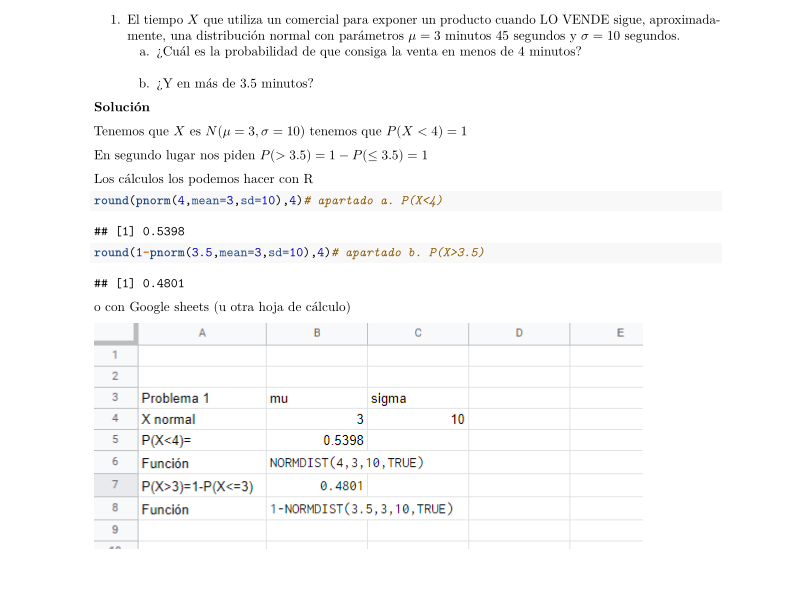
\includegraphics[width=7.61in]{pro1_cont_1}

\newpage

\begin{enumerate}
\def\labelenumi{\arabic{enumi}.}
\setcounter{enumi}{1}
\tightlist
\item
  El tiempo \(X\) que utiliza un comercial para exponer un producto
  cuando NO VENDE sigue, aproximadamente, una distribución normal con
  parámetros \(\mu=2\) y \(\sigma=0.8\).

  \begin{enumerate}
  \def\labelenumii{\alph{enumii}.}
  \tightlist
  \item
    ¿Cuál es el cuantil \(0.95\) de esta variable? Interpretarlo en el
    sentido de tiempo perdido por el comercial.
  \item
    ¿Cuál es el tiempo perdido en el 40\% de las llamadas más cortas?
  \end{enumerate}
\end{enumerate}

\textbf{Solución}

Tenemos que \(X\) es \(N(\mu=2,\sigma=0.8)\) tenemos que buscar el
cuantil \(0.05\) es decir el valor \(x_{0.95}\) tal que
\(P(X <x_{0.95})=0.95\) que es \(x_{0.95}=2\)

En segundo lugar nos piden el cuantil \(x_{0.4}\) es decir el valor
\(x_{0.4}\) tal que \(P(X <x_{0.4})=0.4\) que es \(x_{0.4}=1\)

Los cálculos los podemos hacer con R

\begin{Shaded}
\begin{Highlighting}[]
\KeywordTok{round}\NormalTok{(}\KeywordTok{qnorm}\NormalTok{(}\FloatTok{0.95}\NormalTok{,}\DataTypeTok{mean=}\DecValTok{2}\NormalTok{,}\DataTypeTok{sd=}\FloatTok{0.8}\NormalTok{),}\DecValTok{4}\NormalTok{)}\CommentTok{\# apartado a,  cuantil 0.95}
\end{Highlighting}
\end{Shaded}

\begin{verbatim}
## [1] 3.3159
\end{verbatim}

\begin{Shaded}
\begin{Highlighting}[]
\KeywordTok{round}\NormalTok{(}\KeywordTok{qnorm}\NormalTok{(}\FloatTok{0.4}\NormalTok{, }\DataTypeTok{mean=}\DecValTok{2}\NormalTok{,}\DataTypeTok{sd=}\FloatTok{0.8}\NormalTok{),}\DecValTok{4}\NormalTok{)}\CommentTok{\# apartado b.  cuantil 0.4}
\end{Highlighting}
\end{Shaded}

\begin{verbatim}
## [1] 1.7973
\end{verbatim}

o con Google sheets (u otra hoja de cálculo)

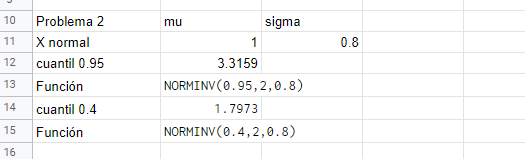
\includegraphics[width=7.29in]{pro2_cont_1}

\newpage

\begin{enumerate}
\def\labelenumi{\arabic{enumi}.}
\setcounter{enumi}{2}
\tightlist
\item
  Un centro de atención telefónica por voz (\emph{call center}) recibe
  por termino medio 102 llamadas por hora. Suponed que el tiempo entre
  llamadas consecutivas es exponencial.

  \begin{enumerate}
  \def\labelenumii{\alph{enumii}.}
  \tightlist
  \item
    Sea X el tiempo entre dos llamadas consecutivas ¿cuál es la
    distribución de \(X\)?
  \item
    Calcular la probabilidad que pasen al menos 2.5 minutos hasta
    recibir la primera llamada.
  \item
    Calcular la probabilidad que pasen menos de 3 minutos hasta recibir
    la siguiente llamada.
  \item
    Calcular la esperanza y la varianza de \(X\).
  \end{enumerate}
\end{enumerate}

\textbf{Solución}

\begin{enumerate}
\def\labelenumi{\alph{enumi}.}
\item
  En 60 minutos recibe 100 llamadas así que en un minuto recibe
  \(\lambda=\frac{102}{60}=1.7\). Luego \(X=\) tiempo entre dos llamadas
  consecutivas en minutos sigue una ley \(Exp(\lambda=1.7)\)
\item
  \(P(X>2.5)=1-P(X\leq 2.5)=0.0143.\)
\item
  \(P(X<3)=P(X\leq 3)=0.9939.\)
\item
  \(E(X)=\frac{1}{\lambda}=\frac{1}{1.7}=0.5882\) y
  \(Var(X)=\frac{1}{\lambda^2}=\frac{1}{1.7^2}=0.346.\)
\end{enumerate}

Cálculos con R

\begin{Shaded}
\begin{Highlighting}[]
\KeywordTok{round}\NormalTok{(}\DecValTok{1}\OperatorTok{{-}}\KeywordTok{pexp}\NormalTok{(}\FloatTok{2.5}\NormalTok{,}\DataTypeTok{rate=}\FloatTok{1.7}\NormalTok{),}\DecValTok{4}\NormalTok{)}\CommentTok{\# apartado b.}
\end{Highlighting}
\end{Shaded}

\begin{verbatim}
## [1] 0.0143
\end{verbatim}

\begin{Shaded}
\begin{Highlighting}[]
\KeywordTok{round}\NormalTok{(}\KeywordTok{pexp}\NormalTok{(}\DecValTok{3}\NormalTok{,}\DataTypeTok{rate=}\FloatTok{1.7}\NormalTok{),}\DecValTok{4}\NormalTok{)}\CommentTok{\# apartado c.}
\end{Highlighting}
\end{Shaded}

\begin{verbatim}
## [1] 0.9939
\end{verbatim}

o con Google sheets (u otra hoja de cálculo)

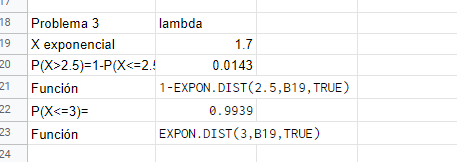
\includegraphics[width=6.35in]{prob3_cont_1}

\newpage

\begin{enumerate}
\def\labelenumi{\arabic{enumi}.}
\setcounter{enumi}{3}
\tightlist
\item
  Sea \(X\) una variable aleatoria normal con parámetros \(\mu=1\) y
  \(\sigma=1\). Calculad el valor de \(b\) tal que
  \(P\left((X-1)^2\leq b\right)=0.1\).
\end{enumerate}

\textbf{Solución}

La v.a. \(X\) es \(N(\mu=1,\sigma=1)\) nos piden \(b\) tal que
\(P((X-1)^2\leq b)=0.1)\),. Notemos que \(b>=0\), además sabemos que
\(Z=\frac{X-\mu}{\sigma}=\frac{X-1}{1}=X-1\) sigue una distribución
\(N(0,1)\).

Tenemos que
\(P((X-1)^2\leq b)=P(-\sqrt(b)\leq (X-1)\leq\sqrt{b})=P(-\sqrt(b)\leq Z\leq \sqrt{b})=F_Z(\sqrt{b})-F_Z(-\sqrt{b})=F_Z(\sqrt{b})-(1-F_Z(\sqrt{b}))= 2*F_Z(\sqrt{b})-1\).

Entonces buscamos \(b\) tal que \(2*F_Z(\sqrt{b})-1=0.1\) y de aquí
tenemos que

\(F_Z(\sqrt{b})=\frac{1+0.1}{2}=0.55\) luego \(\sqrt{b}=z_{0.55}\) y
\(b=\sqrt{z_{0.55}}\) donde \$z\_\{0.55\} es el cuantil \(0.55\) de una
normal estándar \(P(Z\leq z_{0.55})=0.55.\) En definitiva
\(b=\sqrt{z_{0.55}}=\sqrt{0.1257}=0.3545.\)

Para el cálculo del cuantil \(z_{0.55}\) con R es

\begin{Shaded}
\begin{Highlighting}[]
\NormalTok{z0}\FloatTok{.55}\NormalTok{=}\KeywordTok{round}\NormalTok{(}\KeywordTok{qnorm}\NormalTok{(}\FloatTok{0.55}\NormalTok{,}\DecValTok{0}\NormalTok{,}\DecValTok{1}\NormalTok{),}\DecValTok{4}\NormalTok{)}
\NormalTok{z0}\FloatTok{.55}
\end{Highlighting}
\end{Shaded}

\begin{verbatim}
## [1] 0.1257
\end{verbatim}

\begin{Shaded}
\begin{Highlighting}[]
\KeywordTok{round}\NormalTok{(}\KeywordTok{sqrt}\NormalTok{(z0}\FloatTok{.55}\NormalTok{),}\DecValTok{4}\NormalTok{)}
\end{Highlighting}
\end{Shaded}

\begin{verbatim}
## [1] 0.3545
\end{verbatim}

\newpage

\begin{enumerate}
\def\labelenumi{\arabic{enumi}.}
\setcounter{enumi}{4}
\tightlist
\item
  Sea \(Z\) una variable aleatoria \(N(0,1)\). Calcular
  \(P\left(\left(Z-\frac{1}{4}\right)^2 >\frac{1}{16}\right)\).
\end{enumerate}

\textbf{Solución}

\begin{eqnarray*}
P\left(\left(Z-\frac{1}{4}\right)^2 >\frac{1}{16}\right)&=& 1-P\left(\left(Z-\frac{1}{4}\right)^2 \leq \frac{1}{16}\right)\\
&=&
1-P\left(-\sqrt{\frac{1}{16}}\leq Z-\frac{1}{4}\leq\sqrt{\frac{1}{16}} \right)\\
&=&
1-P\left(-\frac{1}{4}+\frac14\leq Z\leq  \frac{1}{4}+\frac14\right)\\
&=&
1-P(0\leq Z\leq 0.5 )=1-(P(Z\leq 0.5)-P(Z\leq 0))\\
&=& 1-(0.6915-0.5)=
0.8085.
\end{eqnarray*}

\newpage

\begin{enumerate}
\def\labelenumi{\arabic{enumi}.}
\setcounter{enumi}{5}
\tightlist
\item
  Un contratista de viviendas unifamiliares de lujo considera que el
  coste en euros de una contrata habitual es una variables \(X\) que
  sigue una distribución \(N(\mu=600000,\sigma=60000)\)

  \begin{enumerate}
  \def\labelenumii{\alph{enumii}.}
  \tightlist
  \item
    ¿Cuál es la probabilidad de que el coste del edificio esté entre
    560000 y 660000 euros?
  \item
    0.2 es la probabilidad de que el coste de la vivienda supere ¿qué
    cantidad?
  \item
    ¿Cuál es el coste mínimo del 5\% de las casa más caras?
  \end{enumerate}
\end{enumerate}

\textbf{Solución}

\begin{enumerate}
\def\labelenumi{\alph{enumi}.}
\tightlist
\item
  \(P(560000\leq X\leq 660000)=P(X\leq 660000)-P(X\leq 560000)=0.8413-`round(pnorm(560000,mean=600000,sd=60000),4)`.\)
\end{enumerate}

Con R

\begin{Shaded}
\begin{Highlighting}[]
\KeywordTok{round}\NormalTok{(}\KeywordTok{pnorm}\NormalTok{(}\DecValTok{660000}\NormalTok{,}\DataTypeTok{mean=}\DecValTok{600000}\NormalTok{,}\DataTypeTok{sd=}\DecValTok{60000}\NormalTok{)}\OperatorTok{{-}}\KeywordTok{pnorm}\NormalTok{(}\DecValTok{560000}\NormalTok{,}\DataTypeTok{mean=}\DecValTok{600000}\NormalTok{,}\DataTypeTok{sd=}\DecValTok{60000}\NormalTok{),}\DecValTok{4}\NormalTok{)}
\end{Highlighting}
\end{Shaded}

\begin{verbatim}
## [1] 0.5889
\end{verbatim}

En el 58\% de los casos (aproximadamente) el coste se tituará entre esas
dos cantidades

\begin{enumerate}
\def\labelenumi{\alph{enumi}.}
\setcounter{enumi}{1}
\tightlist
\item
  Nos piden el valor \(x_0\) tal que \(P(X>x_0)=0.2\), es decir el valor
  que supera el 20\% de las viviendas más caras. Este valor será el que
  deje por debajo el coste del 89\% de las casas por lo que es el
  cuantil 0.8 lo calculamos con R (ejercicio utiliza google sheets para
  obtener el mismo resultado)
\end{enumerate}

\begin{Shaded}
\begin{Highlighting}[]
\KeywordTok{qnorm}\NormalTok{(}\FloatTok{0.8}\NormalTok{,}\DataTypeTok{mean=}\DecValTok{600000}\NormalTok{,}\DataTypeTok{sd=}\DecValTok{60000}\NormalTok{)}
\end{Highlighting}
\end{Shaded}

\begin{verbatim}
## [1] 650497.3
\end{verbatim}

El 20\% de las casas más caras cuestan por encima de 650500 euros
aproximadamente.

\begin{enumerate}
\def\labelenumi{\alph{enumi}.}
\setcounter{enumi}{2}
\tightlist
\item
  Ahora somos más ambiciosos y que remos gastar para estar entre el 5\%
  de casas más caras. De manera similar al caso anterior queremos
  calcular el cuantil \(x_{0.95}\), lo haremos con R
\end{enumerate}

\begin{Shaded}
\begin{Highlighting}[]
\KeywordTok{qnorm}\NormalTok{(}\FloatTok{0.95}\NormalTok{,}\DataTypeTok{mean=}\DecValTok{600000}\NormalTok{,}\DataTypeTok{sd=}\DecValTok{60000}\NormalTok{)}
\end{Highlighting}
\end{Shaded}

\begin{verbatim}
## [1] 698691.2
\end{verbatim}

El 5\% de viviendas más costosas supera los 699000 euros aproximadamente

Con Google sheets (u otra hoja de cálculo)

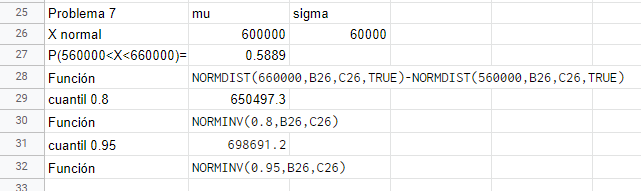
\includegraphics[width=8.9in]{prob7_cont_1}

\newpage

\begin{enumerate}
\def\labelenumi{\arabic{enumi}.}
\setcounter{enumi}{6}
\tightlist
\item
  Si \(X\) está distribuida uniformemente en \((0,2)\) e \(Y\) es una
  variable exponencial con parámetro \(\lambda\). Calcular el valor de
  \(\lambda\) tal que \(P(X<1)=P(Y<1)\).
\end{enumerate}

\textbf{Solución}

\(X\) sigue una ley \(U(0,2)\) luego \(F_X(x)=P(X\leq x)=\frac{x}{2}\)
si \(0<x<2\) y la variable \(Y\) es una \(Exp(\lambda)\) luego
\(F_Y(y)=P(Y\leq y)=1-e^{-\lambda\cdot x}\) si \(x>0\).

Luego \(P(X<1)=\frac{1}{2}\) y \(P(Y\leq 1)=1-e^{\lambda\cdot 1}\). POr
lo tanto nos piden el valor de \(lambda\) tal que
\(\frac{1}{2}=1-e^{-\lambda}\).

Así que \(e^{-\lambda}=1-\frac12=0.5\) luego
\(-\lambda=\ln(0.5)=-0.6931472.\) por lo tanto \(\lambda=0.6931472.\)

\end{document}
